TODO Julie. NOTE: Use APA format.
Relevance, Likability (and Concrete/abstract)

We conducted surveys on Amazon Mechanical Turk to judge the quality of colors and palettes generated by \system. The study evaluated the following hypotheses:

\textbf{H1:} Machine-generated colors are perceived to be more topic-relevant than colors chosen randomly from the Protovis palette, a palette available in an industry standard data visualization toolkit. 

\textbf{H2:} Machine-generated palettes are perceived to be more likable and aesthetically pleasing than palettes composed of random Protovis colors.

\subsection{Method}
To test \textit{topic relevance}, we showed 50 participants from Mechanical Turk six options for each topic. Four of them were colors generated by \system. One was a random color picked from the Protovis palette, an industry standard in data visualization. The last choice was none of the above. Participants picked the one choice that they felt best suited the topic.

To test \textit{palette likability}, we wanted to test if we can combine colors from different football teams, like Cardinal, Cal Bears, and others to create a single, cohesive palette. We hypothesized that the algorithm can choose palettes that are liked better than random palettes. We weren�t sure of the best way to pick one color, so we tried four variations. One tried to pick the most frequent color, another optimized for saturation, one maximized perceptual distance between the colors, and the last picked colors from the topic at random. 
We asked 49 participants from Mechanical Turk to rate our four variations and one randomly generated palette, from Protovis on a scale of 1-7.

We drew topics the topics tested in both studies from six different categories. We classified these categories as being either concrete or abstract. Concrete categories involved tangible objects, and included football teams, sodas, and fruits. Abstract categories involved ideas or concepts that do not have a concrete existence, and included emotions, academic disciplines, and countries. 

\subsection{Results}
\subsubsection{Topic Relevance} 
We found that the \system colors were preferred significantly over the random Protovis colors and none of the above ($\chi^2$(2, N=50) = 83.76, $p <$ 0.001). 947 times out of 1200, Turkers picked a \system color.  Thus, \system is able to pick at a set of colors for a topic that contains at least some appropriate colors.

\begin{center}
\scalebox{0.15}{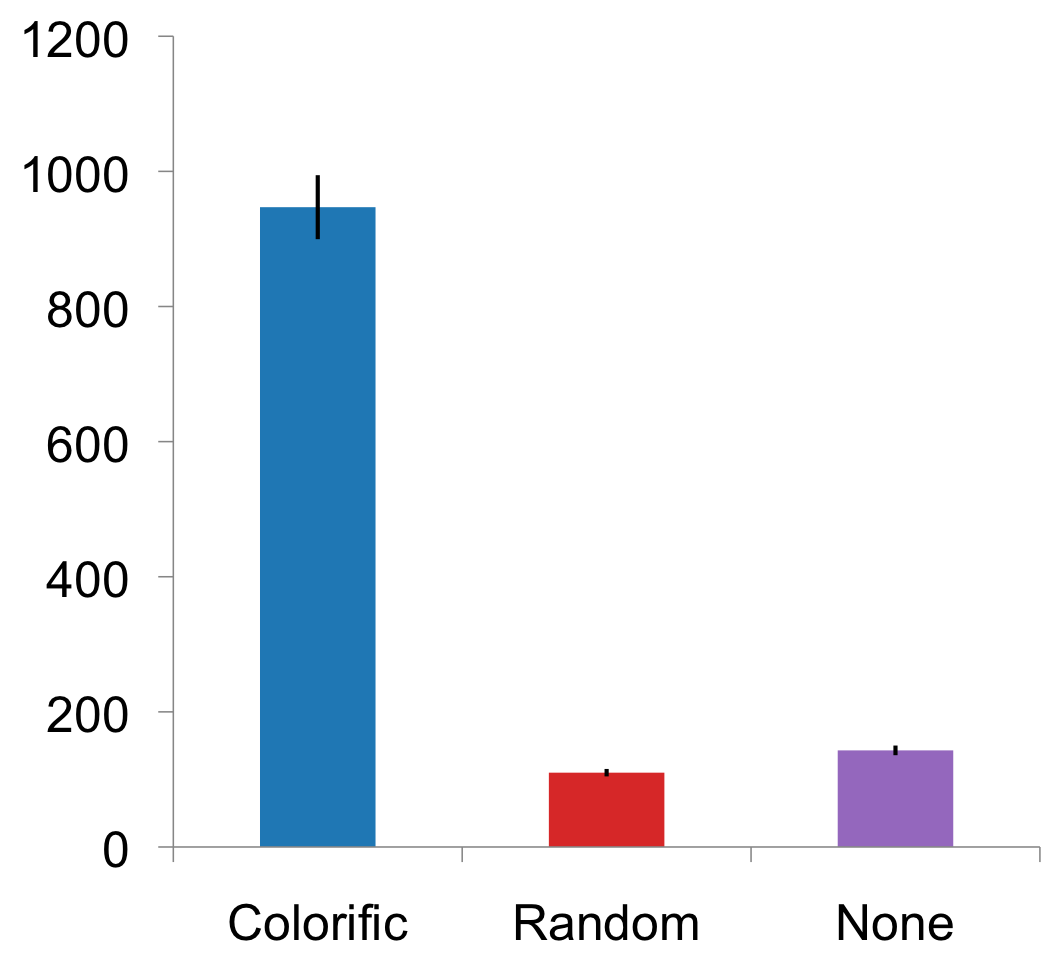
\includegraphics{relevance_chart.png}}
\end{center}

\subsubsection{Palette Likability by Algorithm} 
A Friedman test revealed a significant effect of the type of algorithm used to generate the palettes on rating ($\chi^2$(4)=15.40, $p <$ 0.005). A post-hoc test using Wilcoxon signed-rank tests showed the significant differences between frequency and Protovis palettes ($p <$ 0.05, r = -0.117) and between distance and Protovis palettes ($p <$ 0.05, r = -0.142).

\subsubsection{Palette Likability by Category}
A Friedman test revealed a significant effect of the palette category on rating ($\chi^2$(5)=37.51, $p <$ 0.001). However, when we grouped the categories by concrete or abstract, the results were not significant. Although some palette categories significantly perform better than others, it is not because categories are concrete or abstract. 

\begin{center}
\scalebox{0.5}{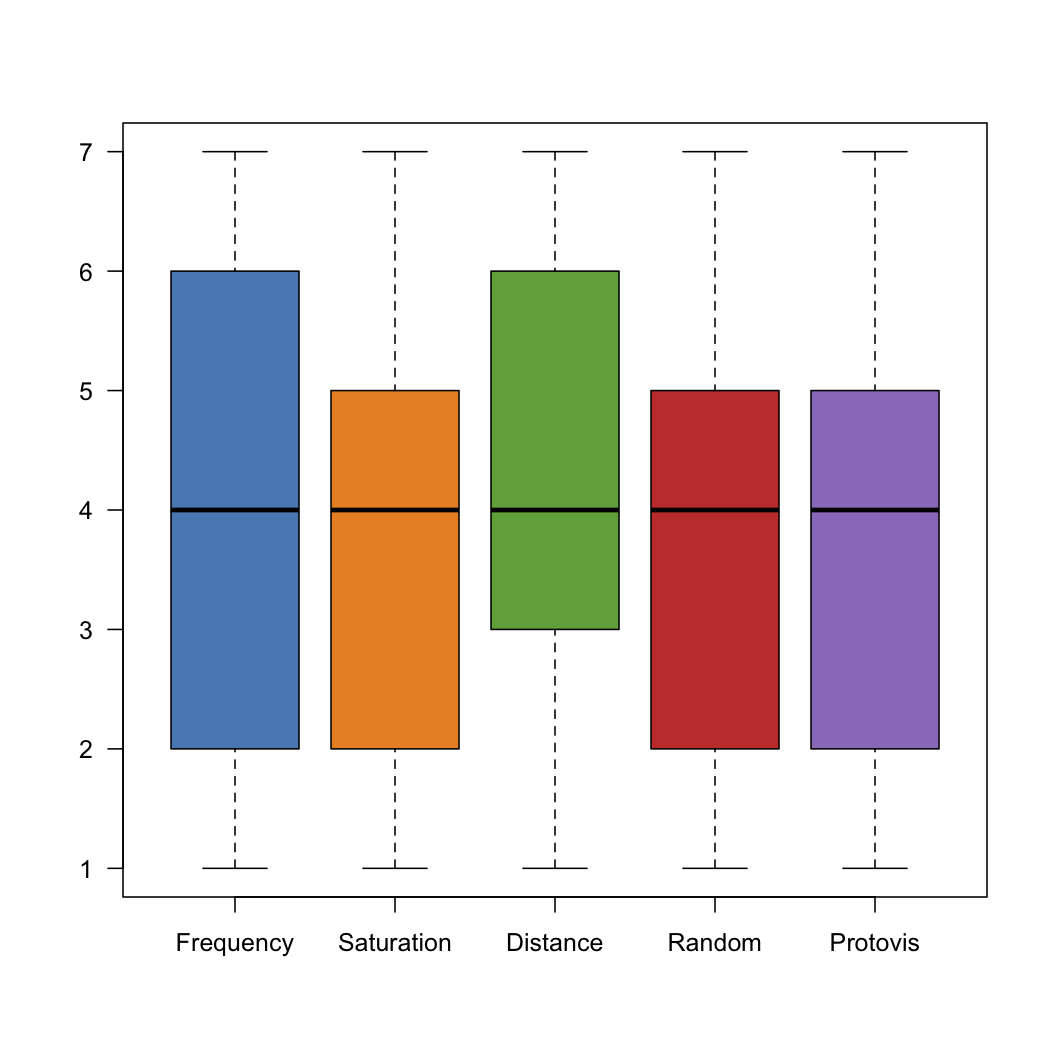
\includegraphics{likability_algorithm.png}}
\end{center}